% --- Title block ---
\begin{center}
  {\LARGE\bfseries rvLLM: Measured Gemma 4 Runtime Throughput\par in Rust on NVIDIA H100\par}
  \vspace{0.6em}
  {\large Andy Norris (m0at), solidSF, Inc.\par}
  \vspace{0.3em}
  {\normalsize\texttt{https://github.com/solidsf-inc/rvLLM}\par}
  \vspace{0.3em}
  {\normalsize San Francisco, April 19, 2026; revised July 14, 2026\par}
\end{center}
\vspace{1em}

% --- Abstract ---
\begin{abstract}
rvLLM is a Rust runtime for Gemma 4 inference. This revision reports a public
rvLLM v0.3.0 H100 measurement against one model revision, one sm\_90 release
archive, and a public receipt set.

\textbf{Measured H100 path.}
In a synthetic fixed-geometry forward sweep, the forced CUTLASS projection
route reached a median 7,492 candidate outputs/s at batch 512; the forced
cuBLASLt projection route reached 6,356, a 17.9\% difference. This is an
internal route comparison, not a comparison with another serving engine.

\textbf{Measurement boundary.}
The timed loop starts at the transformer layers, includes the language-model
head and argmax, and reuses a persistent residual buffer initialized to zero
once before warmup. Decode geometry and metadata remain fixed. It does not
embed input tokens, feed the selected token back, advance position or context,
or generate a valid sequence.

\textbf{Design and validation.}
The path uses FP8 E4M3 weights, Hopper-specific projection kernels,
FlashAttention-3 on sliding-attention layers, fused operations, CUDA graph
replay, and batching. The receipts do not isolate the contribution of each
mechanism. Correctness evidence is limited to published release-gate summaries
for build, parity, ABI, sanitizer, archive, and server smoke.
\end{abstract}

\section{Scope}

rvLLM v0.3.0~\citep{rvllm2026release} is an accelerator-oriented inference
runtime with a native Rust serving path. Its public validation target is one
NVIDIA H100 SXM 80 GB at
sm\_90. Metal and vision source are present but end-to-end generation and
real-weight parity are not asserted for those paths. XLA/TPU work is
experimental and no TPU server is included in this release.

This paper answers three narrow questions. First, what work does rvLLM execute
in the measured fixed-geometry forward? Second, which design choices target
efficient execution on Hopper? Third, what exactly was measured and checked in the
v0.3.0 release? It deliberately does not claim model-quality improvement,
end-to-end serving throughput, or superiority over another inference engine.

The April paper reported older GPU and TPU results. Those GPU rows were later
withdrawn after revalidation found invalid KV-page and block-table geometry.
This revision replaces them with the public v0.3.0 H100 receipt set and does
not carry forward TPU performance claims that lack raw receipts and immutable
model revisions.

\section{Runtime design}

The serving path starts in \texttt{rvllm-serve}, which validates the local HTTP
request and submits bounded work. \texttt{rvllm-runtime} constructs the batch
plan and executes the model step. Loader, metadata, and memory crates validate
model tensors, layouts, and device storage; attention, fused-operation,
CUTLASS, kernel, graph, and sampling crates own accelerator execution. Missing
or incompatible accelerator artifacts are errors rather than silent
fallbacks.

The model is loaded before generation. Prefill processes prompt tokens and
populates the paged KV cache. Ordinary decode then advances one token per
sequence per step; the optional speculative path verifies chunks of draft
tokens. Each transformer layer applies normalization, Q/K/V projection,
rotary position encoding and KV update, attention, output projection,
feed-forward projection, activation, and residual updates. Final
normalization, the language-model head, and sampling produce the next token.

Paged KV state removes the requirement that each sequence occupy its own
contiguous KV region while using one preallocated device arena. Slot mappings,
sequence lengths, block tables, and graph replay inputs must be refreshed
together. This follows the general memory-management motivation of
PagedAttention~\citep{kwon2023pagedattention}, while the public rvLLM
implementation and its supported geometry are release-specific.

\section{How rvLLM targets speed}

\subsection{Less weight traffic and Hopper-specific matrix work}

The measured model stores linear weights in FP8 E4M3 and retains the KV cache
in F16. Relative to BF16, FP8 reduces the bytes moved for the weight matrices and
maps to Hopper tensor-core execution; the format and scaling tradeoffs are
described by Micikevicius et al.~\citep{micikevicius2022fp8}. rvLLM loads the
model's channel scales explicitly and exposes two internal linear-algebra
routes: CUTLASS channel-scale kernels and cuBLASLt. CUTLASS provides the
template machinery used to specialize matrix multiplication for the target
architecture~\citep{nvidia2026cutlass}. The forced route changes channel-scale
transformer projection GEMMs. The language-model head remains on cuBLASLt, and
the remaining forward work is shared.

The two routes do not have one universal winner. In the measured sweep,
cuBLASLt leads at batches 1, 8, and 32; CUTLASS leads at batches 64 through
512. This crossover is the concrete reason to keep route choice explicit and
shape-aware. The receipt does not show that an autotuned policy selected these
winners in the measured forward path: the published policy is a deterministic
baseline, and the channel-scale execution path does not consume its resolved
plans. The paper therefore reports both forced routes rather than an invented
``automatic winner'' result.

\subsection{Attention, fusion, and launch amortization}

The H100 bundle uses FlashAttention-3 for sliding-attention layers; global
attention layers use the validated \texttt{fa\_sm89\_*} fallback path.
FlashAttention-3 uses Hopper asynchrony and low-precision support to improve
attention execution efficiency~\citep{shah2024flashattention3}. rvLLM also
fuses operations such as Q/K/V preparation, normalization and residual work
where the release kernel inventory provides a fused entry point. These choices
are intended to reduce intermediate traffic and the number of separately
scheduled operations. The context length in the public throughput sweep is one
token, however, so that sweep is not an attention-scaling experiment and cannot
quantify the benefit of FlashAttention-3 at long context.

Every timed sample uses CUDA graph capture. A graph records a launch workflow
for replay, reducing repeated host setup and exposing the workflow as a unit to
the CUDA runtime~\citep{nvidia2026cudagraphs}. The graph, model state, and
device buffers are established before timing. The receipts do not include a
graph-on versus graph-off ablation, so graph replay is a documented mechanism,
not a separately measured percentage improvement.

Batching is the final visible lever. Each repeated fixed-geometry forward computes
one argmax candidate per batch row. The benchmark records per-sample aggregate
candidate rate as

\begin{equation}
  T_i = \frac{1000B}{t_i},
\end{equation}

where $B$ is batch size and $t_i$ is sample $i$'s measured step time in
milliseconds. The release summary reports the median of the resulting $T_i$
values. Larger batches amortize fixed launch and weight-movement costs and
expose more matrix parallelism. The observed rise from 46.7 to 7,492 candidate
outputs/s on the CUTLASS route is consistent with that mechanism, but it is
fixed-geometry aggregate throughput rather than sequence generation or per-request
latency.

\section{Measurement method}

The receipt set is labeled July 13, 2026 and accompanies the v0.3.0 release.
It reports the source, model, kernel bundle, driver, toolchain, and harness
parameters shown in Table~\ref{tab:environment}. The model is
\texttt{RedHatAI/gemma-4-31B-it-FP8-Dynamic} at immutable revision beginning
\texttt{448f20b6eb8b}. The model manifest records an aggregate SHA-256 beginning
\texttt{31d8f68ca323}; the complete values are in the linked receipt set. The
kernel archive and receipt bytes have published SHA-256 values. The
source/model/environment associations are operator-attested: the receipts do
not hash the benchmark executable, and the model manifest does not publish the
file-list/hash procedure behind its aggregate.

\begin{table}[htbp]
  \centering
  \small
  \begin{tabularx}{\textwidth}{@{}lX@{}}
    \toprule
    Item & Reported value \\
    \midrule
    rvLLM source & \texttt{afcad6c0145b4455ce91aca52d5a5de4eb4e1572} \\
    Hardware & NVIDIA H100 SXM 80 GB HBM3, sm\_90 \\
    Driver / CUDA & NVIDIA 555.58.02 / CUDA 12.4 \\
    Toolchain & rustc 1.97.0; nvcc 12.4 \\
    CUTLASS / FA3 & \texttt{da5e086dab31d638} / \texttt{1233b73b6c95340c} \\
    Weight / KV dtype & FP8 E4M3 / F16 \\
    Release archive & \texttt{rvllm-kernels-sm90-afcad6c0145b.zip} \\
    Archive SHA-256 & \scriptsize\texttt{97a8a8de4218733514e493193c4f3182ff5b309bf9225fd135e9b64231e6d250} \\
    \bottomrule
  \end{tabularx}
  \caption{Reported environment and kernel release artifact. The kernel
  archive and receipt bytes are hash-identified; other associations are
  operator-attested~\citep{rvllm2026receipts}.}
  \label{tab:environment}
\end{table}

The benchmark constructs a synthetic fixed-geometry state with one context
position per batch row, block size 32, 1,024 total KV blocks, FP8 E4M3 weights,
F16 KV state, and CUDA graph replay enabled. It zeroes the residual once before
warmup, then reuses that persistent buffer while each repetition starts at the
transformer layers and computes through the final
language-model head and argmax without embedding a token or advancing input,
position, context length, slot mapping, or block metadata. It measures batches
1, 8, 32, 64, 128, 256, and 512. Each sample performs 10 warmup iterations followed by 100 timed
iterations. There are two valid samples per route and batch, except batch 512,
which has three. All 30 samples are retained; none are discarded. The table
reports the median recorded by the release summary. Because a two-sample
median is only a midpoint, the small replicate count is a limitation rather
than a broad statistical characterization.

The timer therefore covers a model-shaped fixed-geometry forward, not valid
autoregressive generation. It does not cover model loading, token embedding,
request parsing, tokenization, prompt prefill, HTTP transport, or sequence-state
updates. The public data are project-produced receipts, not an independent
reproduction. They also omit the arena size, executable hash, run order, clocks,
and power state.

\section{Results}

Table~\ref{tab:throughput} and Figure~\ref{fig:throughput} report the complete
H100 sweep. cuBLASLt leads at the three smallest batches, while CUTLASS leads
from batch 64 onward. The largest measured median is 7,492.040 candidate
outputs/s for CUTLASS at batch 512. At that same batch, cuBLASLt reaches
6,356.098 candidate outputs/s; the relative difference is 17.9\%. This compares
the two forced channel-scale projection routes under the same harness; the
language-model head remains on cuBLASLt and the remaining work is shared. It is
not an rvLLM-versus-vLLM result.

\begin{table}[htbp]
  \centering
  \small
  \begin{tabular}{@{}rrrr@{}}
    \toprule
    Batch & CUTLASS cand./s & cuBLASLt cand./s & Leading route \\
    \midrule
    1   & 46.704    & \textbf{48.768}    & cuBLASLt \\
    8   & 369.495   & \textbf{421.023}   & cuBLASLt \\
    32  & 1,447.185 & \textbf{1,543.125} & cuBLASLt \\
    64  & \textbf{2,764.438} & 2,696.043 & CUTLASS \\
    128 & \textbf{5,048.066} & 4,405.914 & CUTLASS \\
    256 & \textbf{7,186.885} & 5,647.870 & CUTLASS \\
    512 & \textbf{7,492.040} & 6,356.098 & CUTLASS \\
    \bottomrule
  \end{tabular}
  \caption{Median aggregate candidate rate for the synthetic fixed-geometry
  forward. The release summary labels this quantity tokens/s.}
  \label{tab:throughput}
\end{table}

The curve shows diminishing throughput gains after batch 256 on the CUTLASS
route. That observation is specific to this model, target, context, and fixed
geometry. It does not establish the latency or throughput of a production request
mix.

\begin{figure}[htbp]
  \centering
  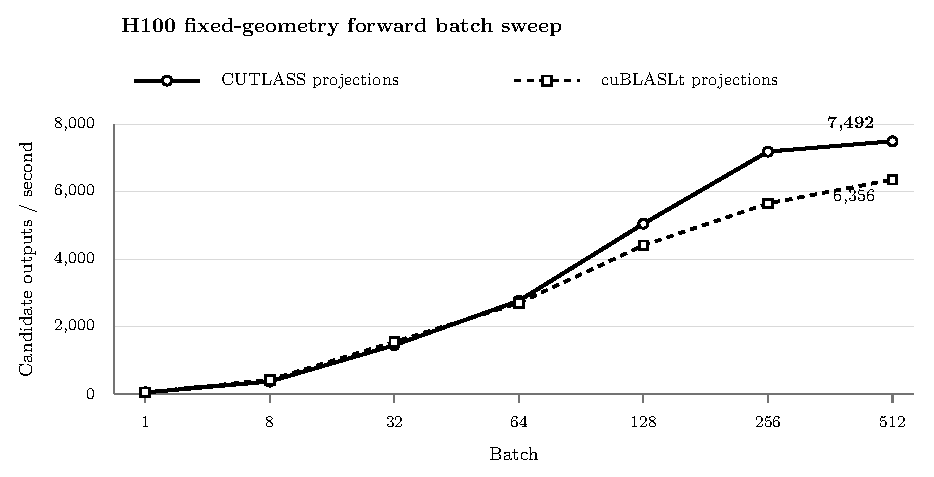
\includegraphics[width=\textwidth]{rvllm-h100-throughput-paper.pdf}
  \caption{The seven-batch sweep from the public release summary. Markers show
  medians; whiskers span the full replicate range. There are two replicates per
  route and batch, except batch 512 with three. Higher aggregate candidate rate
  is better.}
  \label{fig:throughput}
\end{figure}

\section{Correctness and release integrity}

Performance evidence is more useful when release bytes are hash-identified and
the execution path passes numerical and runtime checks. The v0.3.0 validation
summary declares that the final kernel archive was re-extracted and rehashed,
54 files and 48 manifest artifacts were reverified, and deterministic archive
reproduction passed. The source build gates report PASS for clean rebuild, FP8
decode-v2 parity, and FlashAttention-3 sm\_90 parity.

The runtime ABI gate loaded 44 PTX files and resolved 90 PTX entries. Four
shared libraries loaded with 25 expected symbols, four forbidden symbols were
absent, and seven attention-contract values were checked. Compute Sanitizer
reported zero errors and zero leaked allocations. These numbers describe the
published gate result; the public summary and checksums are available, while
the underlying tool transcript is not presented as an independent audit.

The exact-ZIP server-smoke summary reports ten passing checks: health, authenticated status,
model listing, one completion token, one chat-completion token, metrics,
authentication rejection, and rejection of unsupported streaming and stop
requests. The server was observed bound to loopback. The implemented surface
is \texttt{/health}, \texttt{/status}, \texttt{/metrics},
\texttt{/v1/models}, \texttt{/v1/completions}, and
\texttt{/v1/chat/completions}. Generation is non-streaming, only one choice is
accepted, and no Responses endpoint is implemented.

The release semantic audit reviewed 54 package files and scanned 84,504 text
lines. It reports zero credential or secret hits, zero customer or production
infrastructure hits, and zero private-path or solidSF-private-identifier hits. This
is a release-boundary check, not a claim that automated scanning can prove the
absence of every possible disclosure.

\section{Limitations}

The headline number is deliberately narrow. It is aggregate candidate rate from
a synthetic fixed-geometry forward with context-length metadata set to one. No
token embedding occurs. A residual buffer is zeroed once before warmup and then
persists through replay while geometry and metadata remain unchanged; argmax is
not fed back and no valid sequence is generated. The measurement excludes prefill,
networking, request scheduling, and every sequence-state update. It measures one
model revision on one self-reported H100 SXM 80 GB configuration and does not
include a graph ablation, kernel-fusion ablation, power measurement, latency
distribution, or external engine baseline. It also does not evaluate semantic
quality, accuracy, perplexity, or safety of the model output.

The route sweep measures forced CUTLASS and cuBLASLt channel-scale projection
paths. Although a policy
artifact is structurally authenticated and its entries can be launched, the
receipt explicitly states that the current channel-scale Gemma 4 path does not
consume the resolved policy plans. Consequently, this paper makes no claim of
autotuned winner selection in the measured execution.

The retained TPU snapshot in the project benchmark page has no raw receipts or
immutable model revisions and is not used here. Metal, vision, and XLA/TPU
source remain outside the end-to-end release claim. Additional measurements
should cover real prompt distributions, growing contexts, time to first token,
inter-token latency, sustained multi-request serving, and independent
reproduction.

\section{Conclusion}

The measured H100 path combines FP8 weights, Hopper-specific projection kernels,
sliding-layer FlashAttention-3, fused operations, CUDA graphs, and batching. The
synthetic fixed-geometry harness reports 7,492 median candidate outputs/s for
forced CUTLASS projections at batch 512, 17.9\% above the forced cuBLASLt
projection route. No ablation assigns causality, and no valid sequence is
generated. Public hashes cover the kernel archive and receipts; other benchmark
associations are operator-attested. This does not establish autoregressive or
end-to-end throughput, model quality, or cross-engine superiority.

\clearpage
\begingroup
\small
\setlength{\bibsep}{0.35em}
\bibliographystyle{plainnat}
\bibliography{references}
\endgroup
